\section{Smart Contract Idea and Evolution}

Smart contracts represent a milestone in the evolution of blockchain technology. They are electronic transaction protocols that execute the terms of a contract automatically and securely. Contrary to the perception of the term "\textit{smart}", smart contracts do not refer to contracts with artificial intelligence, but rather \textbf{executable programs} based on computer code.

As stated by \textbf{Nick Szabo} \cite{Szabo_1997}, the conceptual pioneer of this innovation:
\begin{quote}
{\Large\textbf{\textcolor{Orange}{“}}}A smart contract is an electronic transaction protocol that executes the terms of a contract. The general objectives are to satisfy common contractual conditions (such as payment terms, liens, confidentiality, and even enforcement), minimize exceptions both malicious and accidental, and minimize the need for trusted intermediaries. Related economic goals include lowering fraud loss, arbitrations and enforcement costs, and other transaction costs.{\Large\textbf{\textcolor{Orange}{”}}} 
\end{quote}
So, in essence, smart contracts promise to make contract processes more efficient, secure, and less burdensome by offering an innovative way to \textbf{automate and ensure the enforcement of contract terms}.

As with blockchain, smart contracts represent a combination of technologies that humans have created in their history. Below is a nice timeline (We hope the font will not make you ask, "\textit{Who lives in a pineapple under the sea?}"\img{tikz/chapter4 - Sponge.png}):

\vspace{-0.5cm}
\begin{figure}[!htbp]
\centering
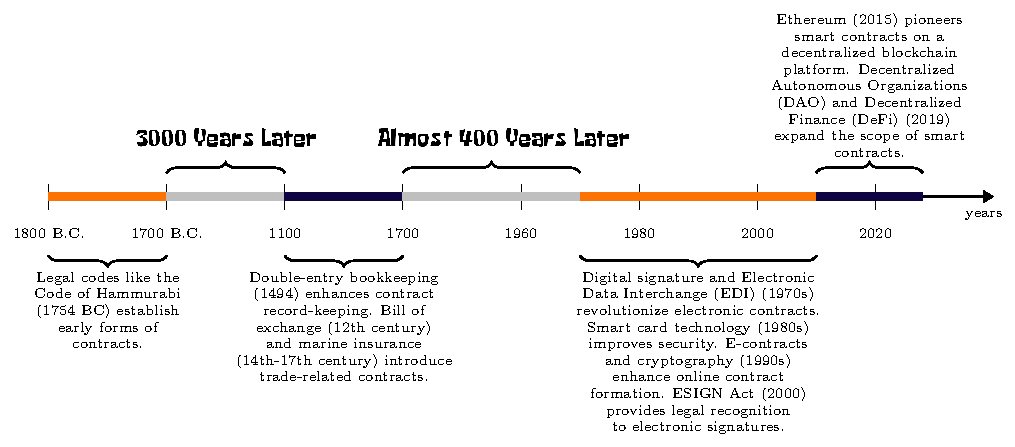
\includegraphics[width=\linewidth]{tikz/chapter4 - Smart Contract Timeline.pdf}
\caption{Smart Contracts Key Inventions Timeline}
\end{figure}


So what is different from a normal contract? In traditional contracts, the verbal text on paper is interpreted by human beings or lawyers ("wet" code). Their legal enforceability is subject to the \textbf{discretionary compliance and semantic flexibility} of human contracts. So, legal validity depends on the willingness of the parties involved to abide by the rules and the ability to interpret the text flexibly and adaptable to the situation.
On the other hand, smart contracts are rules and contracts executed as in a distribution machine ("dry" code). They are legally binding in a technological way, being contracts executed inexorably by code (as \textbf{Lessig} argues: "\textit{code is law}" \cite{les99}), which \textbf{cannot be violated and proceed unstoppably even if conditions have changed}.

\section{Ricardian Contracts}
A Ricardian contract is a legal document that is \textbf{comprehensible and accepted by both humans and machines}, and that is linked to all anticipated future operations (transactions). This type of contract possesses several distinctive properties. First, it is offered by an issuer to holders and represents a right of value managed by the issuer. It is easily readable by people, like a contract on paper, but is also interpretable by programmes, like a database. The contract is digitally signed and contains keys and server information, as well as being associated with a unique and secure identifier. This is basically an \textbf{evolution of the original contract}, indeed each contract can be represented by a graph of objects in prose, interacting in an ecosystem.

\textit{But hey, to really paint the picture, what sets it apart from a smart contract?} Ricardian Contracts focus primarily on being a primary document for the issuance of a digital asset, with an emphasis on \textbf{richer semantics}. In contrast, Smart Contracts are \textbf{more oriented towards programmability} and follow a deterministic approach. So, while Ricardians aim to provide a comprehensive document that is easily understood by all parties involved, Smart Contracts put more emphasis on automating contractual activities through code.

\textit{Let's put it in terms of desserts: Ricardian contracts are like grandma's homemade apple pie - wholesome, comforting, and always a crowd-pleaser. Smart contracts, on the other hand, are more like molecular gastronomy - innovative, impressive, but you're not entirely sure if it's still food...}

\section{Bitcoin or Ethereum? \texorpdfstring{\faBitcoin}{} \ \texorpdfstring{\faEthereum}{}}

Ethereum and Bitcoin differ significantly in their ability to execute smart contracts. \textbf{\textcolor{Orange}{Bitcoin}}, using a full non-Turing script language, is \textbf{limited in its ability to handle complex contracts} or sophisticated decentralised applications. On the other hand, \textbf{\textcolor{Orange}{Ethereum}} offers a \textbf{more powerful environment for smart contracts} through the Solidity language, running on its \textbf{Ethereum virtual machines} (EVMs), which are full Turing. This allows developers to create much more sophisticated smart contracts on Ethereum, with the ability to perform a wide range of calculations or programmable logic. In short, Ethereum offers a more flexible and powerful platform for smart contract development than Bitcoin.
